\documentclass[professionalfonts]{beamer}
\newif\ifanswers
%\answerstrue % comment out to hide answers
\answersfalse
\usepackage[familydefault,light]{Chivo} 
\usepackage[T1]{fontenc}
\usenavigationsymbolstemplate{}
\usepackage[]{hyperref}
\usepackage{tikz,pgf,pgfarrows,pgfnodes,pgfbaseimage}
\graphicspath{{./Pics/}}
\usetikzlibrary{shapes}
\usepackage{setspace}
\newcommand{\evi}[1]{{\colorbox{yellow!50}{{#1}}}}
\newcommand{\exe}[1]{{\color{black!50}{{#1}}}}
\newcommand{\kw}[1]{{\colorbox{black!30}{\color{white}{#1}}}}
\tikzstyle{nd}=[circle,draw=black,thick,minimum size=.8cm,inner sep=1pt]
\setbeamercovered{transparent}
\usetheme{Singapore}
\tikzstyle{nodo}=[ellipse,draw=black!60,fill=black!10,line width=.7pt,minimum width=.7cm,minimum height=.4cm]
\usecolortheme[named=gray]{structure}
\setbeamercolor{block title}{bg=black!20,fg=black}
\setbeamercolor{block body}{bg=black!10,fg=black}

\ifanswers
\title{Algoritmi Numerici (Parte I)}
\subtitle{[Esercitazione 2] Numeri Interi $\mathbb{Z}$ e Complemento a Due}
\else
\title{Numerics (Part I)}
\subtitle{[Exercise Session 2] Integer Numbers $\mathbb{Z}$\\and Two's Complement}
\fi
\date{}
\author{Alessandro Antonucci\\{\tt alessandro.antonucci@supsi.ch}}
%%%%%%%%%%%%%%%%%%%%%%%%%%%%
%\setstretch{1.4}
\begin{document}
    \maketitle
\frame{\frametitle{\ifanswers Un esempio a 4 bit \else A 4-bits example \fi}
    \centering
    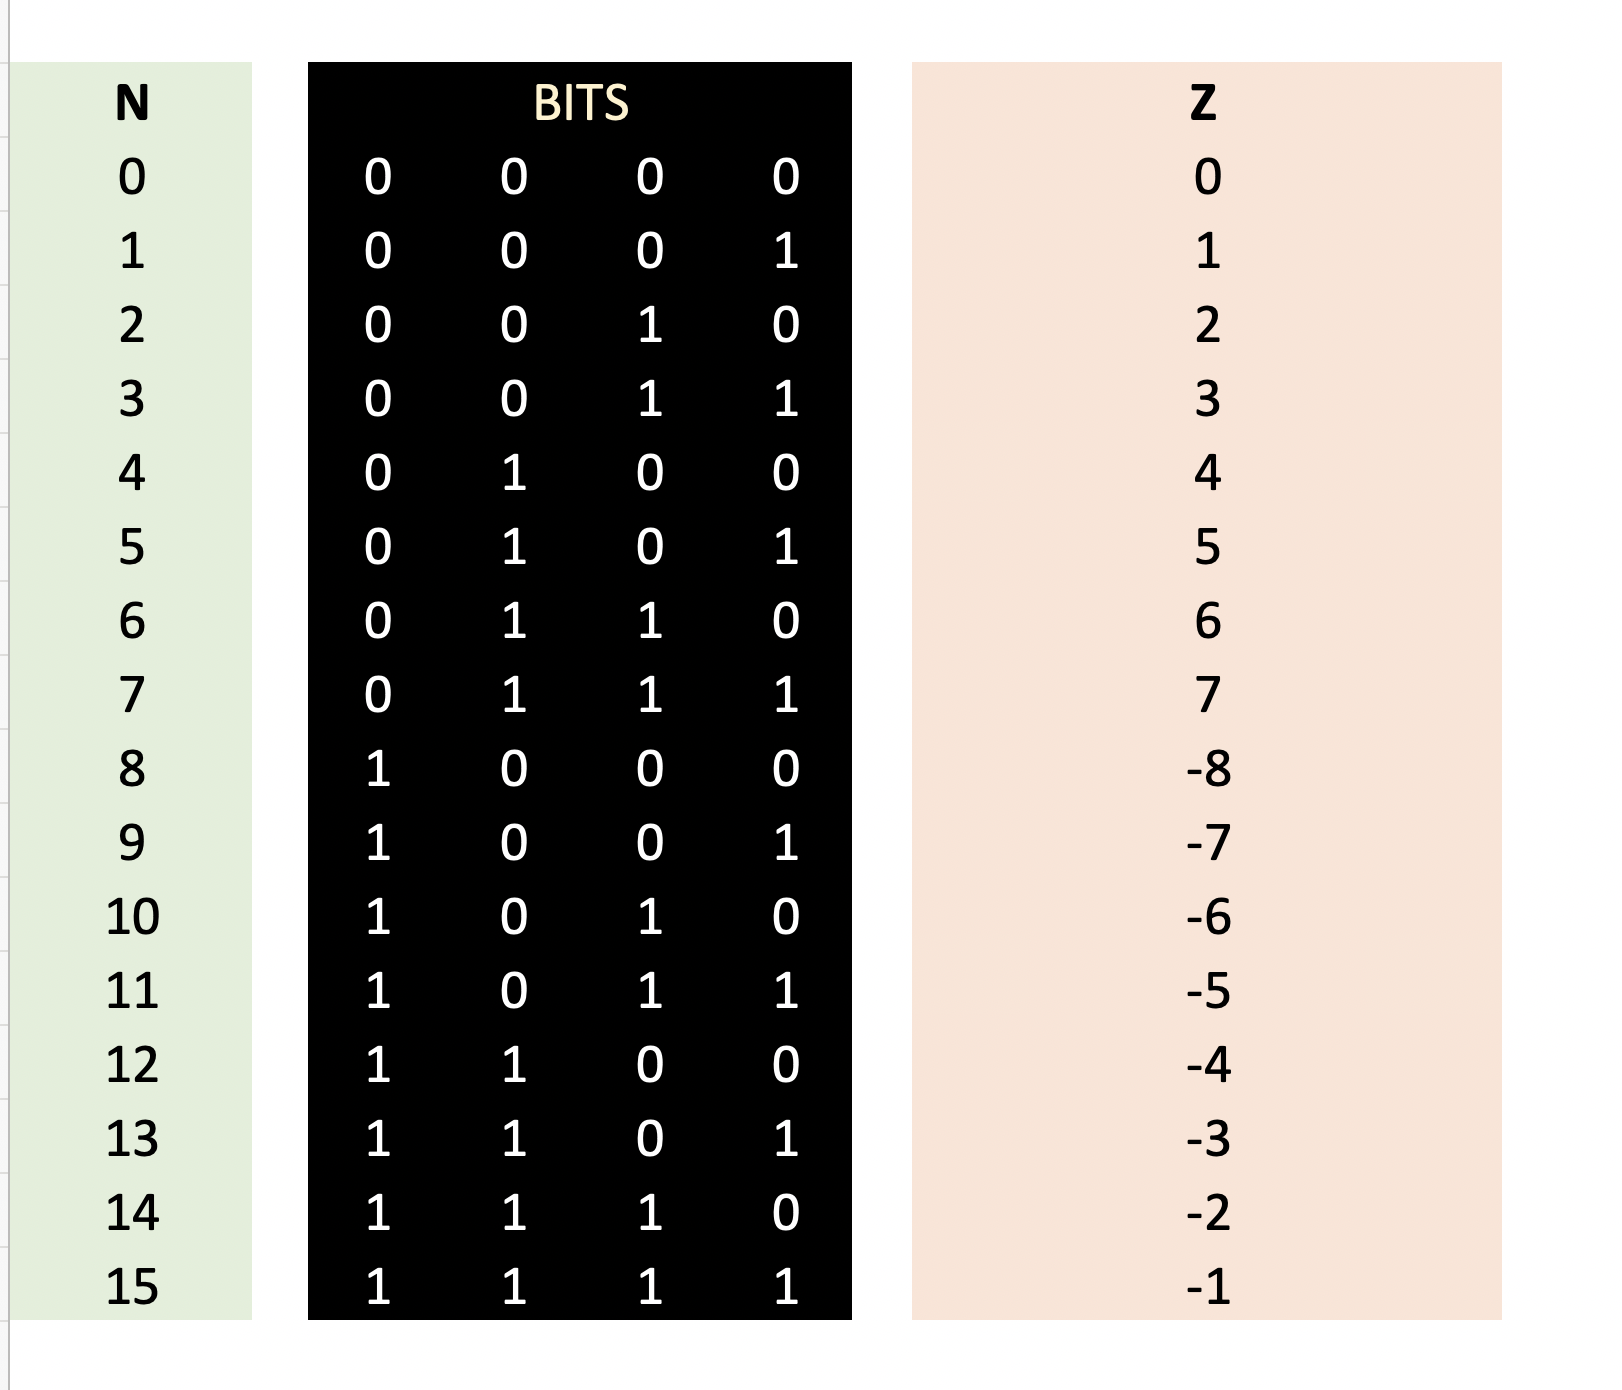
\includegraphics[width=6cm]{z2}\\
\Large
\ifanswers
SI: Pi\`u difficile da capire,\\ma compatto\\e somma in colonna funziona!
\else
YES: Harder to grasp,\\but more compact\\and bitwise sum work!
\fi
}


\frame{\frametitle{\ifanswers Il complemento a 2 \else Two's complement \fi}
\centering
\ifanswers
Linguaggio per rappresentare interi $\mathbb{Z}$ con memorie $n$ bit
\else
Language to represent integers $\mathbb{Z}$ with $n$-bits memories
\fi
\vskip 4mm
\ifanswers
\begin{block}{ALGORITMO DI LETTURA}
\begin{itemize}
\item INPUT = Sequenza di $n$ bits $(b_1,\ldots,b_n)$
\item IF primo bit $=0$
\item THEN OUTPUT = HORNER($(b_1,\ldots,b_n)$)
\item ELSE OUTPUT = - ($2^n$-HORNER($(b_1,\ldots,b_n)$))
\end{itemize}
\else
\begin{block}{NUMBER READING ALGORITHM}
    \begin{itemize}
        \item INPUT = $n$ bits sequence $(b_1,\ldots,b_n)$
        \item IF first bit $=0$
        \item THEN OUTPUT = HORNER($(b_1,\ldots,b_n)$)
        \item ELSE OUTPUT = - ($2^n$-HORNER($(b_1,\ldots,b_n)$))
    \end{itemize}
\fi
\end{block}

\begin{itemize}
\item 0111$\ldots$1 \ifanswers \`e il pi\`u grande positivo \else biggest positive number \fi
\item 1000$\ldots$0 \ifanswers \`e il pi\`u piccolo negativo \else smallest negative number \fi
\item Range $\{-2^{n-1},-1,0,+1,\ldots,2^{n-1}-1\} \subset \mathbb{Z}$
\end{itemize}

}



\frame{\frametitle{\ifanswers Un alternativa per leggere il complemento a 2 \else An alternative reading strategy\fi}
    \centering
    \ifanswers
    \begin{block}{ALGORITMO DI LETTURA (alternativo)}
        \begin{itemize}
            \item INPUT = Sequenza di $n$ bits $(b_1,\ldots,b_n)$
            \item IF primo bit $=0$
            \item THEN OUTPUT = HORNER($(b_1,\ldots,b_n)$)
            \item ELSE 
            \begin{itemize}
            \item Leggi i bit da dx a sx, ricopiali FINCH\`E non trovi un uno
            \item Quando trovi un uno ricopia anche quello, poi NEGA i bit successivi
            \item Chiama sequenza2 il risultato
            \item OUTPUT = - HORNER(sequenza2)
            \end{itemize}
        \end{itemize}
    \end{block}
    \else
    \begin{block}{READING NUMBER ALGORITHM (alternative)}
        \begin{itemize}
            \item INPUT = $n$ bits sequence $(b_1,\ldots,b_n)$
            \item IF first bit $=0$
            \item THEN OUTPUT = HORNER($(b_1,\ldots,b_n)$)
            \item ELSE 
            \begin{itemize}
                \item Read bits from right to left
                \item copy them UNTIL you find a one
                \item If you get the one, copy it, and NEGATE all the others
                \item sequence2 is the result
                \item OUTPUT = - HORNER(sequence2)
            \end{itemize}
        \end{itemize}
    \end{block}
    
   
    \fi
    
    \vskip 4mm
    \ifanswers
    \emph{\`E una sottrazione $2^n$-numero fatta direttamente in base 2}
    \else
    \emph{Automatic base-2 subtraction $2^n$-number}
    \fi
    \vskip 4mm
    \ifanswers
    NEGA(0)=1 e NEGA(1)=0
    \else
    NEGATE(0)=1 and NEGATE(1)=0
    \fi
}


\frame{\frametitle{\ifanswers Dal numero ai bit \else From numbers to bits \fi}
\begin{minipage}[t]{8cm}
\ifanswers
Rappresentare $-34$\\col complemento a 2 a 8 bit
\else
8-Bits two's complement of $-34$
\fi
\vskip 4mm
$-34 = -(2^8-x) \Rightarrow x=2^8-34=222$
\vskip 4mm
$-34 \to$ invhorner(222) $\to 1101 1110$
\end{minipage}
\begin{minipage}[t]{2cm}
{\tiny
222 mod 2 = 0\\
111 mod 2 = 1\\
55 mod 2 = 1\\
27 mod 2 = 1\\
13 mod 2 = 1\\
6 mod 2 = 0\\
3 mod 2 = 1\\
1 mod 2 = 1\\
0}
\end{minipage}}

\frame{
\frametitle{
\ifanswers Esercizio sul complemento a 2 (dai bit al numero)
\else
Two's Complement Exercise (from bits to number)
\fi
}
\Large
\ifanswers
Leggere sequenza di 8 bit (compattata) $F2_{16}$\\ secondo regole complemento a due (ad 8 bit)
\else
Read the sequence of 8 bits ("zipped" in hexadecimal) $F2_{16}$ following the rules of two's complement (for 8 bits sequences)
\fi

\begin{itemize}
\item \ifanswers Metodo 1 \else Method 1 \fi
\begin{itemize}
\item $F2\to 11110010$
\item $HORNER(11110010)=242$
\item output = $-(2^8-242)=-14$
\end{itemize}
\item \ifanswers Metodo 2 \else Method 2 \fi
\begin{itemize}
    \item $F2\to 11110010$
    \item 
    \ifanswers
    Leggo da dx e nego quando trovo 1: $00001110$
    \else
    Reading from right, negating after first one: $00001110$
    \fi
    \item $HORNER(00001110)=14$
    \item output = $-14$
\end{itemize}

\end{itemize}


}


\frame{
\frametitle{\ifanswers Esercizio 1\else Exercise 1\fi}
\begin{itemize}
\ifanswers
\item Il formato {\tt int} rappresenta i numeri interi mediante complemento a due a 32 bit
{\tt short/long int} fanno lo stesso con 16/64 bit
\else
\item Format {\tt int} represents integer numbers by a 32-bit two's complement, formats
{\tt short/long int} are just the same for 16/64 bit sequences
\fi
\ifanswers
\item Eseguire la seguente somma binaria (compattata in esadecimale) ed interpretarla come somma di {\tt short int} (ovvero interi) e di {\tt unsigned short int} (ovvero naturali):
\else
\item Compute the bitwise sum (zipped in hexadecimal) and translate it in a sum of {\tt short int} (= integers) and {\tt unsigned short int} (= natural numbers):
\fi
$$8EE8_{16}+ 2028_{16}$$
\end{itemize}}

\frame{
\frametitle{\ifanswers Soluzione (Esercizio 1) \else Solution (Exercise 1)\fi}
\begin{tabular}{llrlr}
HEXA&\quad \quad BITS&$\mathbb{N}$&$\mathbb{Z}$\\
8EE8+&1000|1110|1110|1000+&36'584&&-28'952\\
2028&0010|0000|0010|1000&8'232&&+8'232\\
\hline
AF10&1010|1111|0001|0000&44'816&&-20'720\\
\end{tabular}}


\frame{
\frametitle{\ifanswers Esercizio 2 \else Exercise 2\fi}
\begin{itemize}
\ifanswers
\item Ricostruire la sequenza di 16 bit che corrisponde al numero $-32'700$ secondo le regole del formato {\tt short int}.
\else
\item Find the 16-bit sequence corresponding to the integer number $-32'700$ as in the {\tt short int} format.
\fi
\item $-32'700 = - (2^{16}-x) \Rightarrow x = 2^{16}-32'700=32'836$
\item 
\ifanswers
Rappresento $x$ in base 2 (appoggiandomi alla base 16)
\else
Representing $x$ in base 2 (using base 16)
\fi
\vskip 2mm
$32'836 \mod 16 = 4$\\
$2'052 \mod 16 = 4$\\
$128 \mod 16 = 0$\\
$8 \mod 16 = 8$
\ifanswers
\item La sequenza \`e $x \to 8044 \to 1000|0000|0100|0100$
\item Sequenza compattata in esadecimale: $8044_{16}$
\else
\item The sequence is $x \to 8044 \to 1000|0000|0100|0100$
\item Sequence zipped in hexa: $8044_{16}$
\fi
\end{itemize}}

\end{document}
